\autsection{Penetrator-Lander Link}{Gustavo Feijóo Carrillo}
%   Through Ice Communications
%       -Scenario and description of operations
%       -Communications during descent
%       -Propagation through ice, ice losses
%       -Link necessary capabilities
%       -Possible hurdles

\paragraph{Link scenario and description of operations}
Three stages in the process of the penetrator descending through the ice crust can be defined to better design the communication system. First, the deployment of the vehicle by lowering it by means of a controlled crane system. In this phase a critical mission operation must be carried out, this is the burial of the lander computer and electronics subsystem to protect it from the surface heavy radiation doses which would shrink the mission life to about a month making it impossible to reach the ocean and carry out the mission goals.

The second phase, would be the penetrator complete buried within the crust and on the melting process to reach the ocean, this might be the longest duration stage depending on the thickness of the crust at the landing site. In this phase, a big risk is the effect of the "slushy" ice trail behind the penetrator. This watery ice would have an increased conductivity and it poses as an obstacle in the path of communication from the penetrator vehicle to the lander. This obstacle mainly affects the antenna pattern characteristics but its effect is greatly dependant on the dimensions of the "slushy" ice trail. On the other hand, a tethered solution would be driven by cable mass necessary for depth goals and to withstand the mechanical forces from being frozen in the ice crust, specially the shear stresses (from sideways motion of ice sheets).

Third, reaching the ocean interface where the main transceiver in the penetrator is left embedded at a safe distance from the interface with the anchoring mechanism for the penetrator and instruments suite. A tether/cable enabled for communications will serve as link from the instruments to the main transceiver and relay the science data and telemetry to surface.

\begin{figure}[htb]
	\centering
	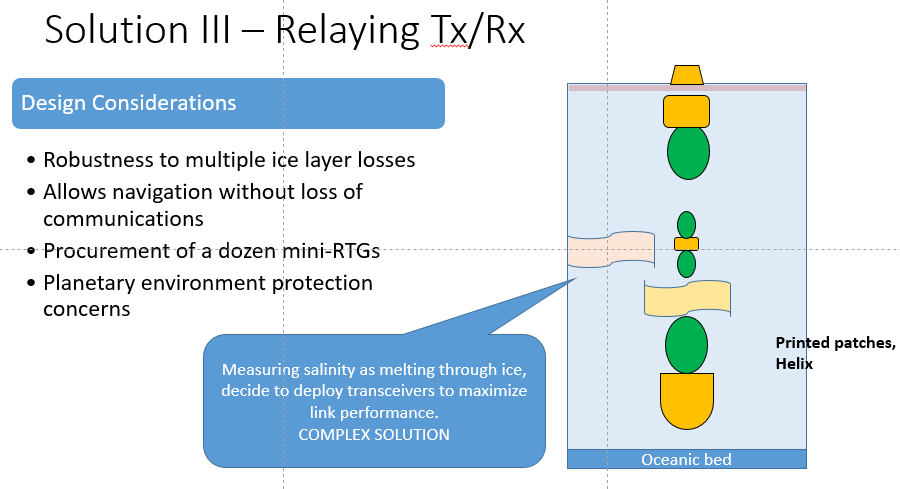
\includegraphics[width=\textwidth]{figures/comms/iceLink-relay}
	\caption{\textit{DRAFT} Through-ice communications.}
	\label{fig:through-ice_comms_relay}
\end{figure}

\subsection{Link Drivers}

\autsubsection{Tethered Link}{Kristian Sloth Lauszus}
One option for the penetrator to surface communication would be to use a tethered link connected from the end of the penetrator to the surface station. For instance a optical fiber could be used. The main benefit when using optical fiber for communication is the huge data rate of 10 Gb/s and beyond, which will allow the penetrator to broadcast scientific data, images and even video to the lander. Another advantage is that it is not unusual for optical fiber communication to work at up to 100 km without the need of any amplification\cite{website:optical_fiber_info}, which is way more than the worst case scenario of 36 km, as described in chapter \ref{sec:structural_profile}. Thus the optical fiber is very interesting, as it will basically allow one to send all the scientific data to the lander with little to any concerns about the data rate.

\subsubsection{Optical fiber strain}

However one major concern is whenever the strain from the ice caused by the tidal waves will exceed the capabilities of the fiber and eventually break it. This will be discussed in detail in the following section.\\

\noindent
According to Hook's law the force along the longitudinal axis of the optical fiber is given by:
\begin{equation}
	 F = k \, \Delta l
\end{equation}
Where $k$ is the elastic constant of the optical fiber and $\Delta l$ is the relative deformation caused by the perturbation force $F$. This law is fulfilled as long as the deformation does not exceed the elastic limit of the optical fiber which will prevent the fiber from retracting back to its original shape.

By knowing the Young's modulus of the optical fiber once can calculate the force of the perturbation using the following formula:
\begin{equation}
	F = E_G \, A \frac{\Delta l}{l}
\end{equation}
Where $E_G$ is the Young's modules, $A$ is the area of the optical fiber and $l$ is the length of the optical fiber.

By measuring the force applied to an optical fiber and plotting it versus the strain one can estimate the Young's modulus at the point where the slope of plot is no longer linear. Furthermore this point will also indicate the maximum strain of a given optical fiber. This strain number is very useful in our case, as this tell us how much the fiber can stretch before it is degraded. A typical number for protected optical fiber is about 3-5 percent\cite{article:optical_fiber_properties,article:optical_fiber_mechanical}. Since the column above the penetrator will start to freeze up again it is very important that the vertical strain of the ice does not exceed this critical value, as this will cause the optical fiber to break.

\subsubsection{Discussion}

Fortunately the vertical strain of the ice sheet on Europa is only estimated to be 0.3 \%, however this does not take into effect any potential cracks that occurs at the ice surface, as described in chapter \ref{sec:surface_studies}. This might cause the ice to shift horizontally, thus risking to break the cable. Thus the tethered link is very risky and should properly not be used as the only form of communication\cite{book:communication}.

The optical fiber could be wound up on a spool with a total weight of only a few kilograms\cite{book:communication}. However the wheel will also add up in complexity of the system and increase the volume. There will also be a risk of the wheel getting stuck while unwinding the optical fiber. Another option would be to use even more rigid cable, but this will increase volume and mass significantly\citet{iceLink-scott}.


\autsubsection{Ice embedded Repeaters link}{Kristian Sloth Lauszus}

Another option for communicating between the penetrator and the lander would be to use multiple transceivers that would get deployed at certain intervals by the penetrator, as it is described by \citet{iceLink-scott}. Thus a series of repeaters was proposed, designed into 10 cm diameter cylinders with a height of 2-3 cm. Each repeater would have a 1 GHz patch antenna in the top and bottom of the cylinder and contain all the needed hardware for transmitting and receiving the data including a RTG for power and heat. Each repeater could also have temperature, pH, salinity, hydrophones and various other sensors embedded.

In the study the goal was to have a data rate of 10 kHz at 400 mW through a 10 km ice crust. In the paper the number of repeaters was found to be heavily influenced by salinity of the ice and temperature profile used. Thus the number of repeaters would increase in salty ice and if a layered ice temperature profile is used compared to a linear ice temperature model (see chapter \ref{sec:IceTemperatureProfile} and \ref{sec:IceTemperatureProfile2}). In the paper the salty ice is assumed to contain 13 PPM (Parts Per Million) salt impurities. For the linear ice temperature model the minimum amount of repeater was found to be 4 for a ice thickness of 3.5 pure ice, while 14 transceivers would be needed for 10 km salty ice. While the number of repeaters needed for the layered ice temperature profile would be vary from 8 for 5 km and 34 for 20 km pure and salty ice respectively.

However as \citet{iceLink-scott} also points out the distance between the receivers could be increased at the cost of a lower data rate, thus if the ice ends up being thicker or more salty than first expected, this could be compensated for by the on-board computer in the penetrator. On the other hand if the ice is more pure the distance could be increased or the data rate increased.

One way for the penetrator to deploy the repeaters would be to make the repeaters buoyant in such a way that they would float upward and align themselves in such a way that the antennas point up and down. A new repeater could then be deployed when the signal strength drops below a certain threshold. One problem with using the repeaters is that the complex dielectric permittivity increase in the order of 1000 times in water compared to ice, thus the penetrator might have to sit and wait for the repeater to freeze if a minimum data rate is needed.

Another option would be to use the repeaters at the outer ice crust where the ice is colder and the risk of fractures in the ice is higher, then once the penetrator gets below a certain depth a tether could be used to connect to the last repeater deployed at the warmer inner ice, where the risk of a tether breaking is less. This is especially useful if the layered ice temperature profile ends up being close to reality, as the temperature of the ice increases significantly in the beginning of the ice sheet, as discussed in chapter \ref{sec:IceTemperatureProfile2}. However then further studies would be needed in order to get more certainty regarding the ice temperature profile of Europa. Also further studies are needed regarding the salinity, as it is critical in order to estimate the number of repeaters needed.


% Wireless links
\autsubsection{Ice embedded wireless communications}{Gustavo Feijóo Carrillo}

In a previous study from JPL's Cryobot concept regarding ice communications \cite{iceLink-scott}, we find the assumption of the communication transceiver relays being allowed to refreeze in the ice but there is no deeper details on this matter. The main subject here is the behaviour of the "slushy ice" or water and ice mixture above the descending penetrator, since this trail has a meaningful effect on the antenna performance of the penetrator communication subsystem as shown in Figures \ref{fig:unaffected}, \ref{fig:smallSlush} \& \ref{fig:bigSlush}. The concentration levels of impurities in the water/ice mixture also has an impact but will be leaved for future works, in the present study a salty water of $15ppt$ is used as a simplified model.

%   Fig. Slush trail diagram
\begin{figure}[htb]
	\centering
	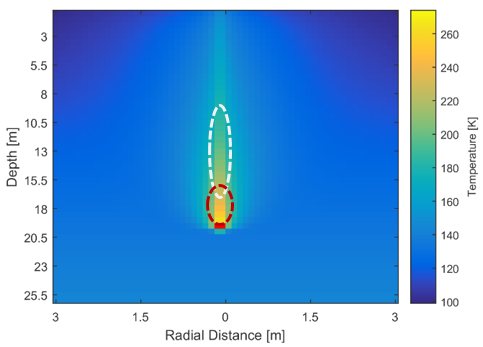
\includegraphics[width=.66\textwidth]{figures/comms/slushTrail}
	\caption{This figure based on the melting profile simulation, it can be seen from the temperature gradient trailing the penetrator that in the close proximity a column of melt water first (red), followed by a mix warm ice and water which is referred as "slush" (white) forms the obstacle discussed in this section. The profile shown spans almost 4 days.}
	\label{fig:through-ice_comms}
\end{figure}

%   Fig. No slush
\begin{figure}[htb]
	\centering
	\subfloat[]{
		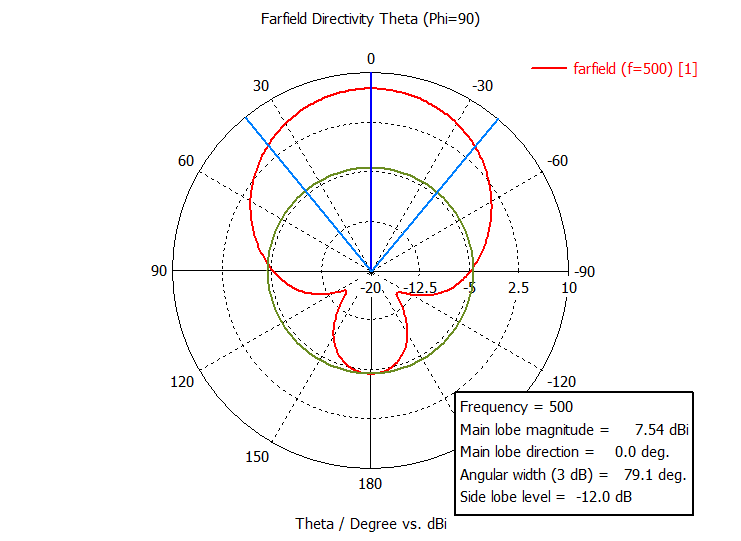
\includegraphics[width=.48\textwidth]{figures/comms/antPattern-cPatchRadome}
		\label{fig:antPatt-patchRadome}
	}
	\subfloat[]{
		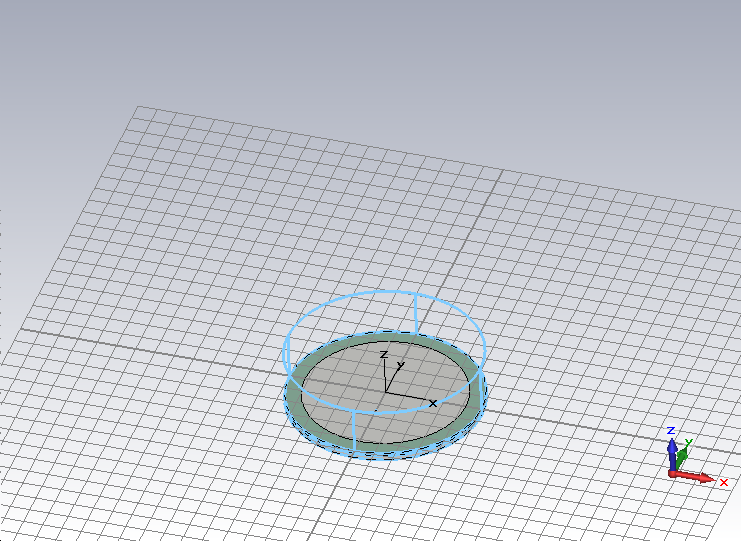
\includegraphics[width=.48\textwidth]{figures/comms/component-cPatchRadome}
		\label{fig:comp-patchRadome}
	}
	\caption{Unaffected antenna pattern.}
	\label{fig:unaffected}
\end{figure}
%   Fig. Small slush
\begin{figure}[htb]
	\centering
	\subfloat[]{
	    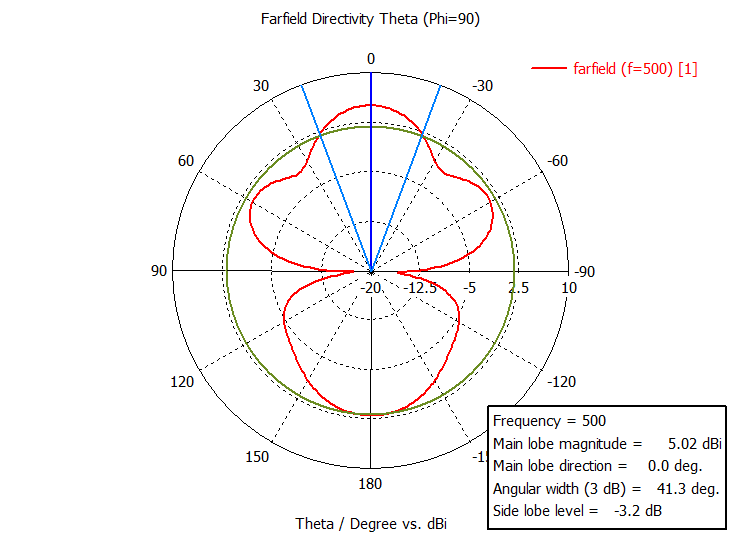
\includegraphics[width=0.48\textwidth]{figures/comms/antPattern-slushEffect-a}
	    \label{fig:slushEffect_a}
	}
	\subfloat[]{
		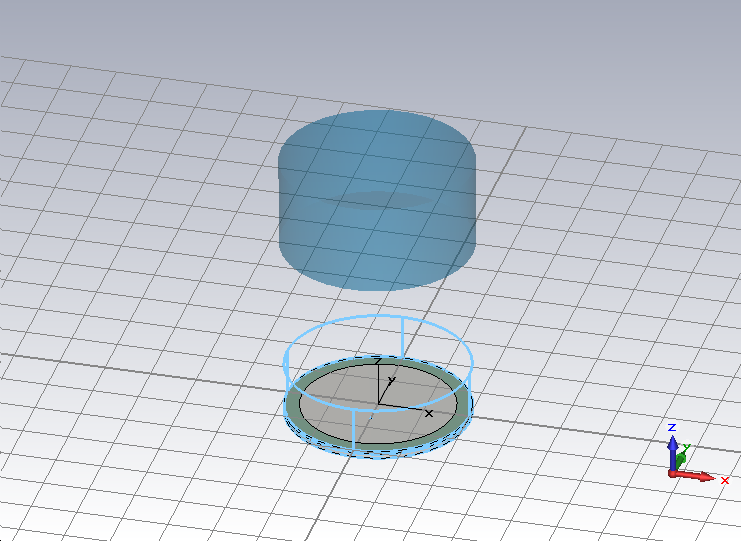
\includegraphics[width=.48\textwidth]{figures/comms/component-slushEffect-a}
		\label{fig:comp-smallSlush}
	}
	\caption{Effect of small watery ice obstacle in antenna path.}
	\label{fig:smallSlush}
\end{figure}
%   Fig. Big slush
\begin{figure}[htb]
	\centering
	\subfloat[]{
	    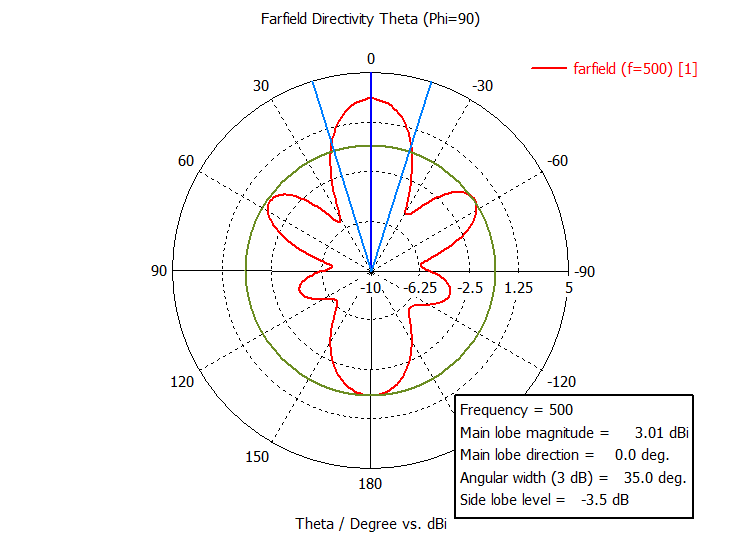
\includegraphics[width=0.48\textwidth]{figures/comms/antPattern-slushEffect-b}
	    \label{fig:slushEffect_b}
	}
	\subfloat[]{
		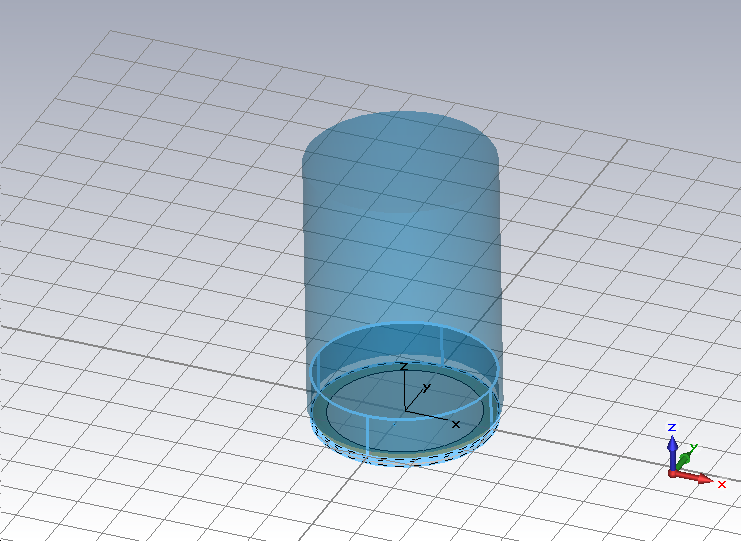
\includegraphics[width=.48\textwidth]{figures/comms/component-slushEffect-b}
		\label{fig:comp-bigSlush}
	}
	\caption{Effect of longer watery ice trail.}
	\label{fig:bigSlush}
\end{figure}


% Effect on link design
\subsubsection{Considerations for Link Sizing and Antenna choice}

\paragraph{High Directivity Link}
\begin{figure}[htb]
	\centering
	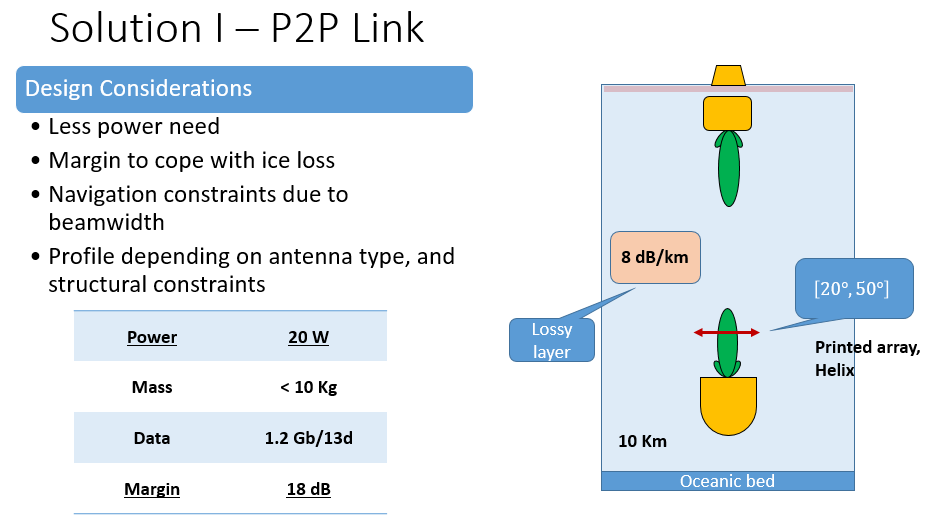
\includegraphics[width=\textwidth]{figures/comms/iceLink-p2p-HighD}
	\caption{ \textit{DRAFT} Sol I.}
	\label{fig:iceLink-p2p-HighD}
\end{figure}

% LD Link
\subsubsection{Low Directivity Link}
\begin{figure}[htb]
	\centering
	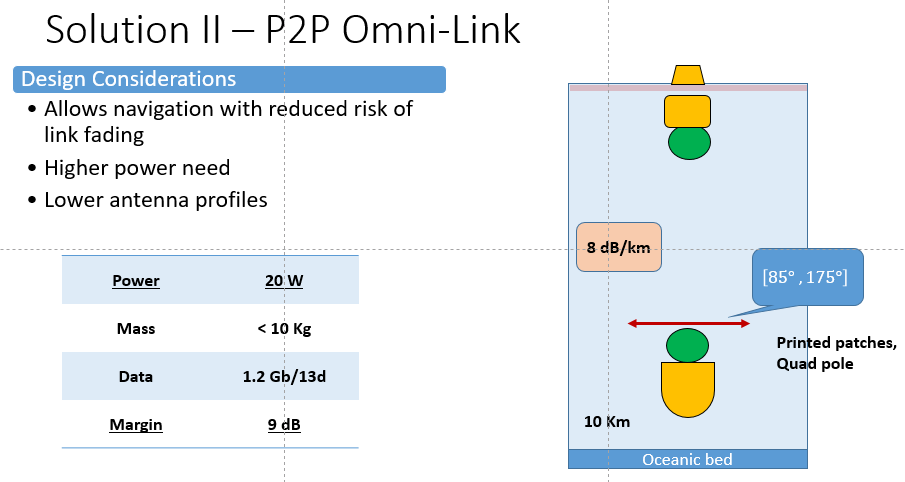
\includegraphics[width=\textwidth]{figures/comms/iceLink-p2p-LowD}
	\caption{ \textit{DRAFT} Sol II.}
	\label{fig:iceLink-p2p-LowD}
\end{figure}

% Ice embedded relays
\subsubsection{Relay Link}
\begin{figure}[htb]
	\centering
	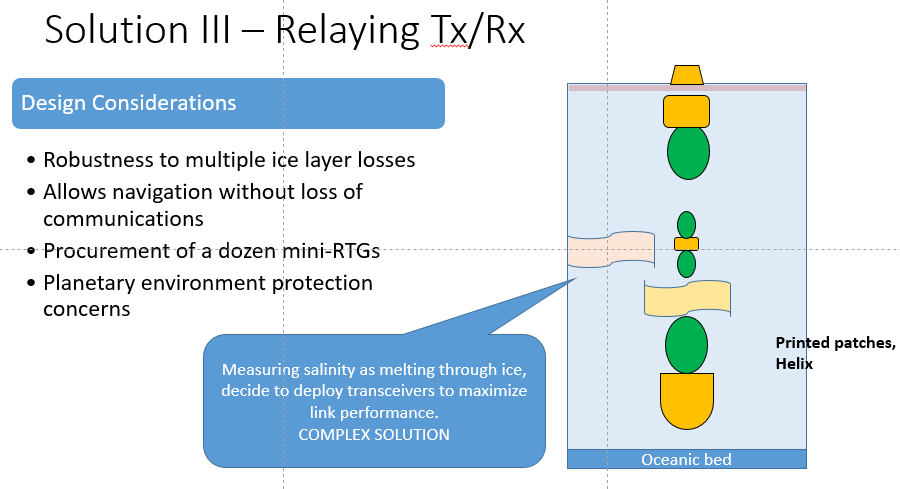
\includegraphics[width=\textwidth]{figures/comms/iceLink-relay}
	\caption{ \textit{DRAFT} Sol III relays.}
	\label{fig:iceLink-relay}
\end{figure}
